\section{Drone Ship Physics Model }

Very important part of my project is to have a good physics model of the drone ship. 
That model will be used to simulate IMU and GPS sensor readings, as well as to provide a realistic environment for testing control algorithms.

First step is to model the buoyancy of the ship. The ship will be modeled as a rigid body with a certain mass, width, length, and draft. Currently model does not assume any particular shape for the ship, but it will be important to consider the shape in future iterations to improve the accuracy of the model. The buoyancy force will be calculated based on the 4 points of the ship: the bow, stern, port, and starboard. The buoyancy force will be calculated as the weight of the displaced water, which is equal to the volume of the submerged part of the ship multiplied by the density of water and gravity. 

Same points will be used to calculate the wave drag force. In each of 4 points there is a wave drag force acting in the normal direction to the surface of the water. Forces are scaled to the size of the ship. 

This approach captures the essential physics of the problem while keeping the model computationally efficient. Placement of these points is visible in the figure below
\ref{fig:ship_buoyancy_points}.


That model will be used to simulate the motion of the ship in response to control inputs and environmental forces. 


\begin{figure}[htbp]
    \centering
    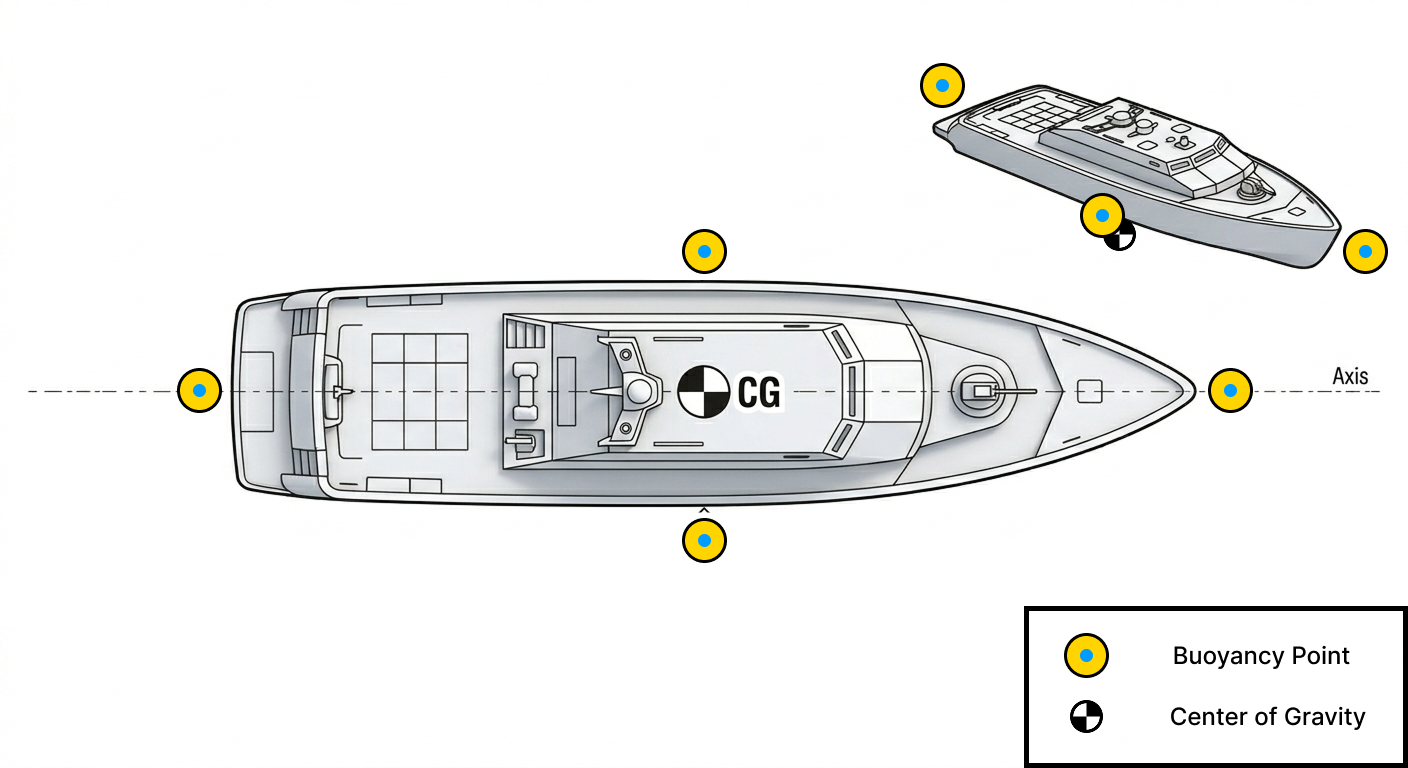
\includegraphics[width=0.8\textwidth]{images/ship_buoyancy.png}
    \caption{Ship buoyancy model diagram.}
    \label{fig:ship_buoyancy_points}
\end{figure}